\documentclass[10pt]{article}
\pagestyle{plain} \setlength{\textwidth}{12cm}
\setlength{\oddsidemargin}{2cm} \setlength{\evensidemargin}{2cm}
\setlength{\textheight}{23cm}
\usepackage{amssymb,latexsym,amsmath,amsthm,verbatim,calc}
\usepackage{graphicx,epsfig,epstopdf,amssymb,color,makeidx,float,caption,sidecap}

\begin{document}
\title{A template for a Math xxx written homework assignment}

\author{Benjamin Kennedy}
\maketitle

\bigskip
\noindent
{\bf Acknowledgements and sources of help}: list acknowledgements/collaborators here.

\bigskip
\noindent
{\bf Problem 1.1 \ \ } Here is some work on a problem called ``Problem 1.1".  When I am writing, I can insert mathematical symbols into my writing with dollar signs: $x^2 - y = 0$.

Special commands in math mode start with backslashes.  Here, for example, are some Greek letters: $\alpha$, $\beta$, $\gamma$, $\delta$, $\epsilon$.

Here is how to make subscripts and superscripts: $x_2^3$.  If the subscript or superscript has multiple characters, enclose it in curly brackets: $x_{2,3}^{\beta}$.

If I want to center a mathematical expression on its own line, I can do so as follows (notice I am also showing you how to use summation notation and fractions here):
\[
\sum_{k = 0}^\infty r^k = \dfrac{1}{1-r}.
\]

Here is how to make a ``low" ellipsis (if you're leaving elements out of a list):
\[
s_1,s_2,\ldots,s_n.
\]
Here is how to make a ``middle" ellipsis (if you're leaving terms out of a sum):
\[
s_1 + s_2 + \cdots + s_n.
\]

Most standard special functions can be named with backslashes, and plain text can be included in math mode with the ``mbox" command.  A backslash by itself creates extra space.
\[
\sin^2(x) + \cos^2(x) = 1 \ \mbox{for any real number} \ x.
\]

Special brackets (like curly brackets) can also be created with backslashes, and ``left" and ``right" commands give them the correct size to enclose what they are suppose to enclose.
\[
\mathbb{Q} = \left\{ \frac{a}{b} \ : \ a \in \mathbb{Z}, \ b \in \mathbb{Z} \setminus \{0\} \right\}.
\]

If you need to write multiple lines of mathematics at once, do it like this.  (The double backslash says where the line break goes, and the ampersands indicate places that should be vertically aligned with each other.)
\begin{align*}
x^2 + 5x + 6 &= 0 \ \Longrightarrow \\
(x+2)(x+3) &= 0 \ \Longrightarrow \\
x = -2 & \ \mbox{or} \ x = -3.
\end{align*}

Here is a system of two linear equations in three variables:
\begin{align*}
2x_1 - 3x_2 + 7x_3 &= 0 \\
x_2 - 10x_3 &= 2
\end{align*}

Sometimes you will want to include a picture in your document.  (NOTE: for this to work in Overleaf, the .pdf file you want to include must be among your ``project" files.)

\begin{center}
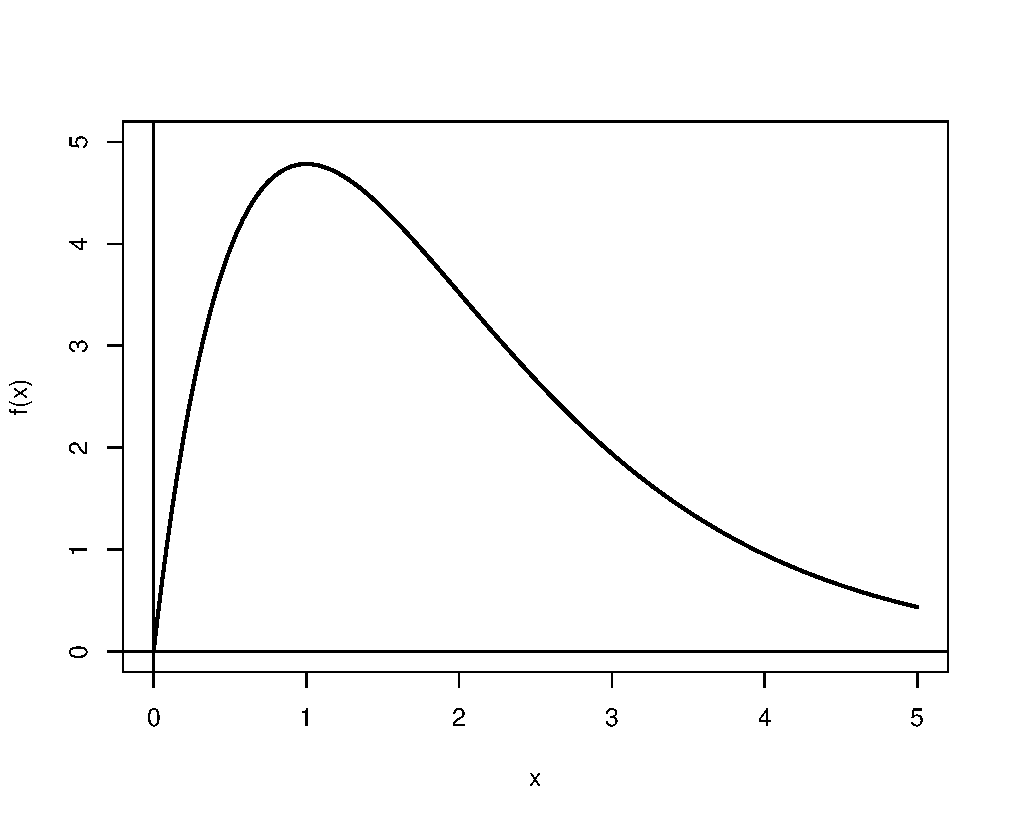
\includegraphics[width = 4in, height = 3in]{TemplateFig1.pdf}
\end{center}

Here is a short theorem with a proof: \emph{Theorem: the sum of two even numbers is even}.

PROOF.  Suppose that $a$ and $b$ are two even numbers.  This means that $a = 2k$ for some integer $k$ and $b = 2n$ for some integer $n$.  We therefore have
\[
a+b = 2k + 2n = 2(k+n).
\]
This shows that $(a+b)$ is of the form $2 \times \mbox{(some integer)}$, which is just what it means for $(a+b)$ to be even.  $\square$

\bigskip
\noindent
{\bf Problem 1.2 \ \ } Here's where I could put work on Problem 1.2!  Here is how to enter a $2 \times 3$ matrix.  The {\tt ccc} in curly brackets means that I want a matrix with three columns where each entry is center in the column.   Entries across a row are separated with ampersands, and the rows are separated with double slashes.  The matrix is enclosed in parentheses.
\[
\left[ \begin{array}{ccc}
1 & 2 & 3 \\
4 & 5 & 6
\end{array} \right]
\]
Here is a matrix multiplication.
\[
\left[ \begin{array}{ccc}
1 & 2 & 3 \\
4 & 5 & 6
\end{array} \right]
\left[ \begin{array}{c}
-1 \\ 0 \\ 1
\end{array} \right]
=
\left[ \begin{array}{c}
2 \\ 2
\end{array} \right].
\]

\bigskip
\noindent
{\bf Additional Problem 1 \ \ } Here's where I could put work on a problem called ``Additional Problem 1"!

\bigskip
\noindent
In the early going, you will want to do a lot of things that you don't know how to do.  Take the time to figure them out --- it's time well spent.  For help, consult:

\begin{itemize}
\item your friends;
\item your faculty;
\item the internet (try a Google search of ``square root symbol in LaTeX").
\end{itemize}

\end{document} 